\chapter{Avaliação dos resultados do experimento}
	\section{ETAPA 1 – Display de 7 segmentos}

		Verificou-se, para todos os casos de entrada, que o valor previsto pela tabela-verdade
		como saída era válido, demonstrando sucesso na implementação do experimento. Isso pode
		ser visualizado tanto pela simulação, como na execução na placa.

		\begin{figure}[H]
			\centering

			\begin{subfigure}[b]{0.44\textwidth}
				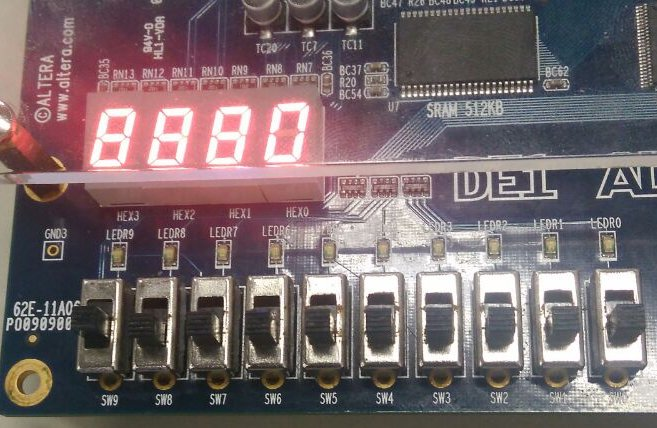
\includegraphics[width=\textwidth]{img/etapa1/0}
				\label{fig:etapa1-0}
				\caption{Número 0}
			\end{subfigure}
			~
			\begin{subfigure}[b]{0.44\textwidth}
				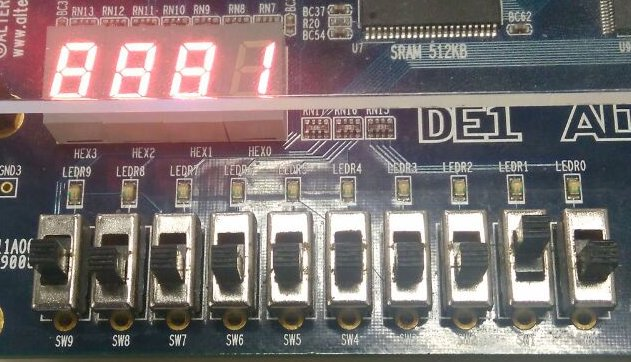
\includegraphics[width=\textwidth]{img/etapa1/1}
				\label{fig:etapa1-1}
				\caption{Número 1}
			\end{subfigure}

			\begin{subfigure}[b]{0.44\textwidth}
				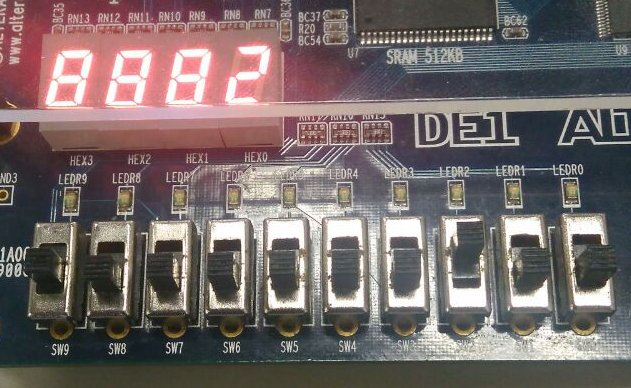
\includegraphics[width=\textwidth]{img/etapa1/2}
				\label{fig:etapa1-2}
				\caption{Número 2}
			\end{subfigure}
			~
			\begin{subfigure}[b]{0.44\textwidth}
				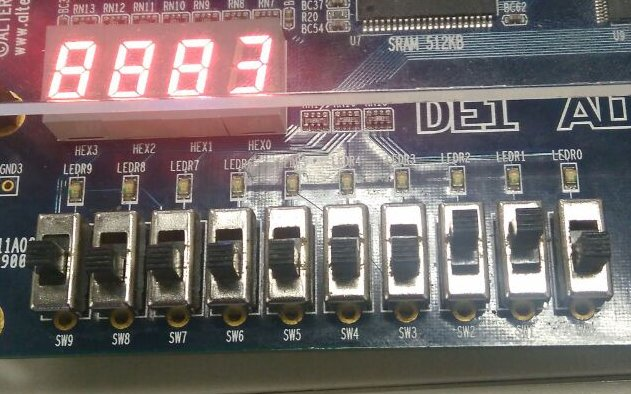
\includegraphics[width=\textwidth]{img/etapa1/3}
				\label{fig:etapa1-3}
				\caption{Número 3}
			\end{subfigure}
			\begin{subfigure}[b]{0.44\textwidth}
				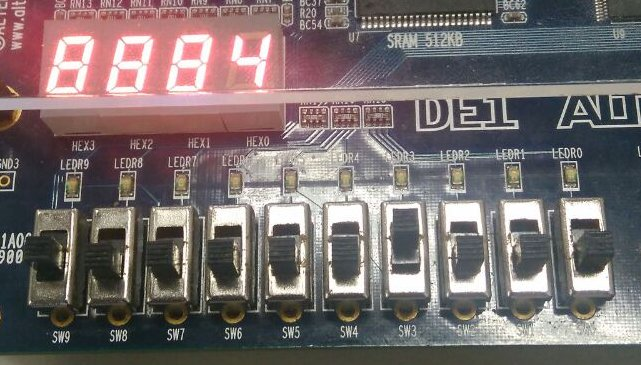
\includegraphics[width=\textwidth]{img/etapa1/4}
				\label{fig:etapa1-4}
				\caption{Número 4}
			\end{subfigure}
			~
			\begin{subfigure}[b]{0.44\textwidth}
				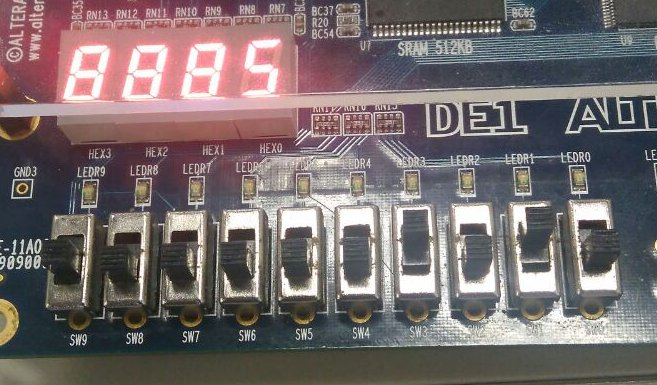
\includegraphics[width=\textwidth]{img/etapa1/5}
				\label{fig:etapa1-5}
				\caption{Número 5}
			\end{subfigure}

			\caption{Teste do circuito rodando na placa, no intervalo de 0-5.}\label{fig:etapa1Teste1}
		\end{figure}

		\begin{figure}[H]
			\centering

			\begin{subfigure}[b]{0.44\textwidth}
				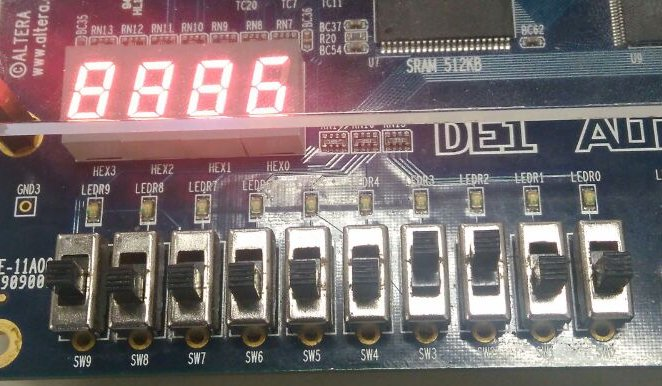
\includegraphics[width=\textwidth]{img/etapa1/6}
				\label{fig:etapa1-6}
				\caption{Número 6}
			\end{subfigure}
			~
			\begin{subfigure}[b]{0.44\textwidth}
				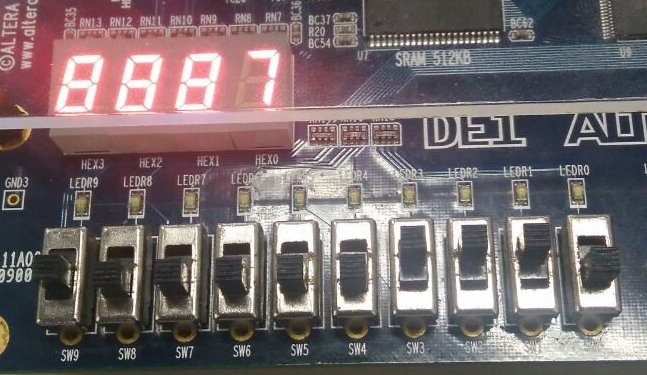
\includegraphics[width=\textwidth]{img/etapa1/7}
				\label{fig:etapa1-7}
				\caption{Número 7}
			\end{subfigure}

			\begin{subfigure}[b]{0.44\textwidth}
				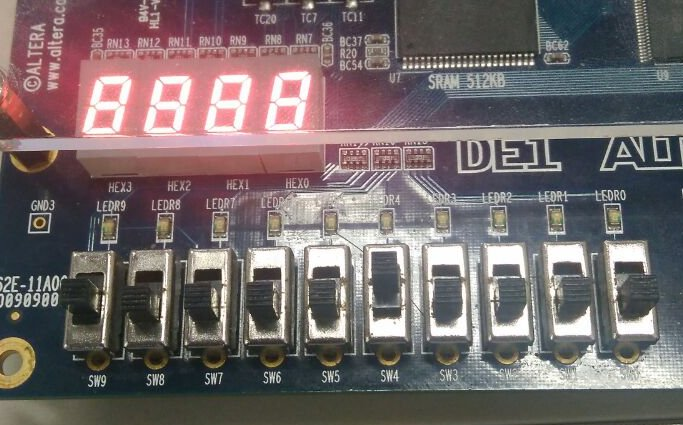
\includegraphics[width=\textwidth]{img/etapa1/8}
				\label{fig:etapa1-8}
				\caption{Número 8}
			\end{subfigure}
			~
			\begin{subfigure}[b]{0.44\textwidth}
				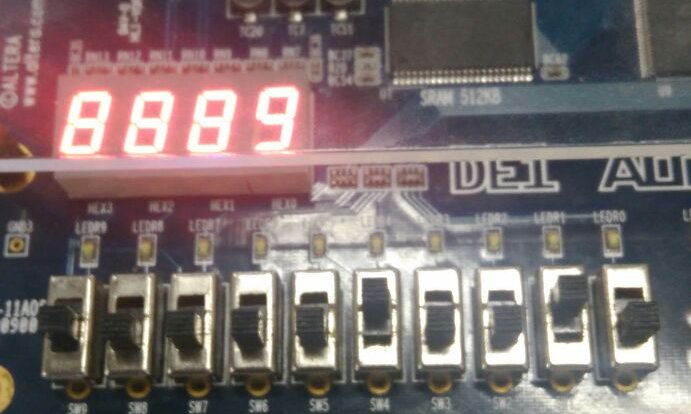
\includegraphics[width=\textwidth]{img/etapa1/9}
				\label{fig:etapa1-9}
				\caption{Número 9}
			\end{subfigure}

			\caption{Teste do circuito rodando na placa, no intervalo de 6-9.}\label{fig:etapa1Teste2}
		\end{figure}

		\begin{figure}[H]
		    \centering
			\caption{\label{fig:etapa1Simulacao}Resultado da simulação da etapa 1.}
			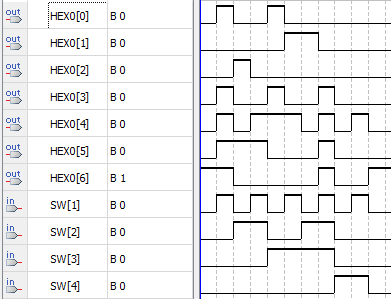
\includegraphics[width=1\textwidth]{img/etapa1/SimulacaoSegmentos7}
		\end{figure}


	\section{ETAPA 2 – Meio-somador 1 bit}
		Na etapa 2, o experimento demonstrou os resultados esperados, de acordo com a
		 \autoref{table:tabelaMeioSomador}.

		\begin{figure}[H]
		    \centering
			\caption{\label{fig:etapa2Simulacao}Resultado da simulação da etapa 2.}
			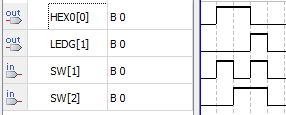
\includegraphics[width=1\textwidth]{img/etapa2/SimulacaoMeioSomador1Bit}
		\end{figure}

		Após o deploy na placa no kit DE1, o kit educacional da Altera, o circuito apresentou
		 os resultados esperados, representando o resultado da soma no display de 7 segmentos HEX0 ,
		e indicando a presença de um \textit{carry} ou não, através do LEDG[1],
		 conforme \autoref{fig:etapa2Teste}.

		\begin{figure}[H]
			\centering

			\begin{subfigure}[b]{0.44\textwidth}
				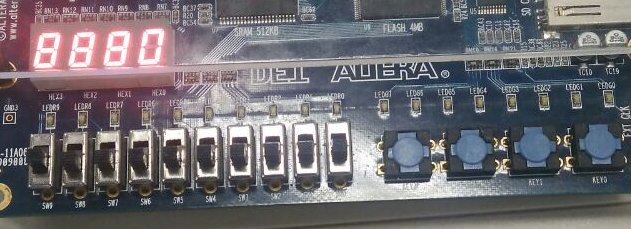
\includegraphics[width=\textwidth]{img/etapa2/00}
				\label{fig:etapa2-00}
				\caption{Entrada 0 0}
			\end{subfigure}
			~
			\begin{subfigure}[b]{0.44\textwidth}
				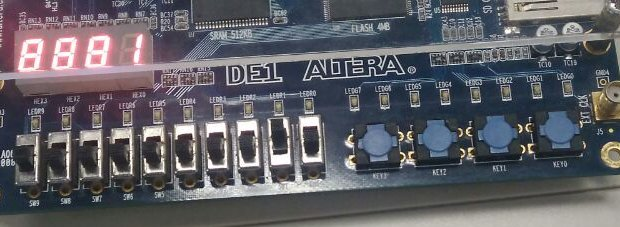
\includegraphics[width=\textwidth]{img/etapa2/01}
				\label{fig:etapa2-01}
				\caption{Entrada 0 1}
			\end{subfigure}

			\begin{subfigure}[b]{0.44\textwidth}
				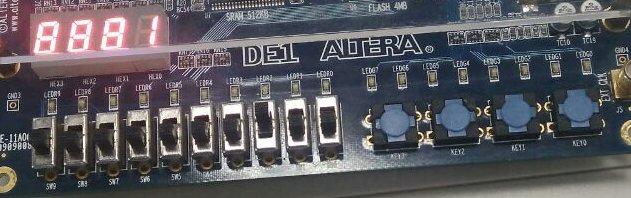
\includegraphics[width=\textwidth]{img/etapa2/10}
				\label{fig:etapa2-10}
				\caption{Entrada 1 0}
			\end{subfigure}
			~
			\begin{subfigure}[b]{0.44\textwidth}
				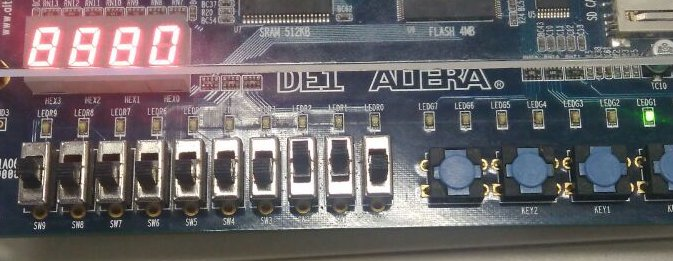
\includegraphics[width=\textwidth]{img/etapa2/11}
				\label{fig:etapa2-11}
				\caption{Entrada 1 1}
			\end{subfigure}

			\caption{Teste do circuito rodando na placa.}\label{fig:etapa2Teste}
		\end{figure}

		Nota: Este diagrama esquemático, diferente do anterior, já foi feito
		utilizando exclusivamente portas NAND, não sendo necessária qualquer metodologia de conversão.
		O circuito utilizado, o TTL 7449, apenas substitui aqui o circuito criado para a implementação
		da etapa anterior, respeitando as expressões do item 2.1. É só um circuito já conhecido que
		cumpre a mesma função que o que foi criado para aquela etapa do experimento.

		\footnote{Para mais detalhes sobre o TTL 7449 acesse o \autoref{anexo:datasheet-7449}.}
	\section{ETAPA 3 – Meio-somador 4 bits}


%Apresentar os resultados da simulação em software e da utilização do Kit DE1 e/ou
%protoboard. Utilizar figuras, descrevê-las e discuti-las.
